\chapter{Introduction à l'apprentissage profond}\label{chap:intro ml}

L'astronomie, l'astrophysique et la cosmologie sont officiellement entrée dans l'ère du \textit{Big Data} en 2020, 
soit une décennie où les scientifiques se noient dans 
un océan de données, maintenant mesuré dans l'ordre du \textit{petabyte}, soit un millions de \textit{gigabytes}, ou $\sim 10^{15}$ \textit{bytes}. 
Par exemple, l'observatoire Vera C. Rubin produira environ 2 \textit{petabyes} de données, soit une quantité de données 
impossible à traiter dans son ensemble pour la plupart des algorithmes utilisés quotidiennement par les physiciens pour inférer les propriétés du ciel 
et de l'Univers; sans parler de la quantité accumulée par l'observatoire au travers des 10 années planifiées pour le relevé astronomique qui doit débuter 
en $2024$ \citep{lsst2009,lsst2021}. 

C'est cette réalité qui nous force à développer des méthodes d'analyses plus sophistiquées pour l'inférence de quantités physiques à partir 
d'images, spectres et vidéos du ciel. C'est aussi ce qui motive l'étude des méthodes liées à l'apprentissage machine, et plus particulièrement 
l'apprentissage profond, qui promettent de simplifier énormément l'analyse statistique des grands ensembles de données à venir. Ce chapitre se veut 
une courte introduction aux concepts de bases liés à l'apprentissage machine. 
La section \ref{sec:bayes} est un survol la théorie des statistiques bayésiennes, dont le but est d'introduire certains concepts cruciaux qui sous-tendent la 
théorie de l'apprentissage machine. Ensuite, les concepts de l'apprentissage machine classique sont décrits à la section \ref{sec:app classique}. 
Les réseaux neuronaux et l'apprentissage profond sont introduits via à la section \ref{sec:app profond} 
comme une généralisation possibles de l'apprentissage machine classique. 
Finalement, on introduit les réseaux de neurones convolutifs à la section \ref{sec:cnn}. 

Pour une discussion plus détaillée des concepts abordés dans ce chapitre, voir les manuels de références \citet{BengioDeepLearningBook,}.

\section{Survol des statistiques bayésiennes}\label{sec:bayes}

L'inférence bayésienne est une théorie statistique qui a pour but principal de modéliser l'état de connaissance, 
ou le degré de croyance, associé à un évènement.  En terme général, l'inférence bayésienne est un processus de mise à jour de nos 
connaissance \textit{a priori}, c.-à-d. nos connaissances avant d'observer un évènement. Étant donné un processus physique auquel on associe une loi de 
vraisemblance, c.-à-d. une loi de probabilité qui dicte la vraisemblance d'observer un évènement particulier, alors le processus d'inférence 
bayésienne correspond simplement à la repondération de nos connaissance par la vraisemblance, ce qui revient à multiplier la loi de 
probabilité \textit{a priori} par la vraisemblance d'un évènement (et renormaliser).

Par exemple, considérons un tirage au sort. 
La vraisemblance d'observer pile ou face est une loi qui modélise la probabilité d'observer un évènement, $y \in \mathcal{Y}=\{0, 1\}$, étant 
donné un paramètre $x \in \mathcal{X} = [0, 1]$ qui contrôle le processus physique, dans ce cas la probabilité d'observer pile ou face. 
Pour cet exemple, la vraisemblance est une loi de Bernoulli 
\begin{equation}
        p(y \mid x) = x^{y} (1 - x)^{1 - y}\, .
\end{equation} 
\textit{A priori}, on associe une probabilité égale (uniforme) au paramètre $x$, soit $p(x) = \mathcal{U}(0, 1)$. 
Ce choix reflète une ignorance complète du processus physique qui contrôle le tirage au sort.
Supposons maintenant qu'on observe $y$, un évènement tiré de la loi physique $p(y \mid x^{\star})$, où $x^{\star}$ est le véritable paramètre de la loi physique.
Le théorème de Bayes nous indique comment ajuster notre degré de croyance, maintenant $p(x \mid y)$, soit la loi \textit{a posteriori} du paramètre $x$ étant donné avoir observé $y$
\begin{equation}\label{eq:Bayes1}
        p(x \mid y) = \frac{p(y \mid x) p(x)}{p(y)} \, .
\end{equation} 
La loi de probabilité $p(y)$, aussi appelée l'évidence, normalise la loi \textit{a posteriori}, qui est proportionnelle au produit de la vraisemblance $p(y \mid x)$ et 
de la loi \textit{a priori} $p(x)$. En pratique, on peut évaluer $p(y)$, une loi marginale, en l'exprimant 
en terme de la loi jointe $p(x, y)$, soit 
\begin{equation}
        p(y) = \int_\mathcal{X} dx\, p(y, x) \, .
\end{equation} 
On peut ensuite utiliser la définition d'une loi conditionnelle 
\begin{equation}
        p(y \mid x) = \frac{p(x,\, y)}{p(x)} \, ,
\end{equation} 
pour exprimer l'évidence, $p(y)$, en terme de la vraisemblance et de la loi \textit{a priori} 
\begin{equation}
        p(x \mid y) = \frac{p(y \mid x) p(x)}{\int_\mathcal{X} dx\, p(y \mid x) p(x)} \, .
\end{equation} 
Supposons maintenant qu'on observe un certains nombre de tirages au sorts
\begin{equation*}
        y_1,y_2,\dots,y_N \overset{\mathrm{i.i.d.}}{\sim} p(y \mid x^{\star})\, ,
\end{equation*}
indépendamment et identiquement distribués ($i.i.d.$) selon la même loi physique, $p(y \mid x^{\star})$. Pour mettre à jour nos connaissances, on procède 
itérativement. En premier lieu, on trouve la distribution \textit{a posteriori} $p(x \mid y_1)$ avec le théorème de Bayes \eqref{eq:Bayes1}. Ensuite, 
on remplace la distribution \textit{a priori}, $p(x)$, par $p(x \mid y_1)$ dans le théorème de Bayes \eqref{eq:Bayes1} 
pour obtenir la loi \textit{a posteriori}, $p(x \mid y_1, y_2)$. Et ainsi de suite.
Puisque les observations sont $i.i.d.$, alors ce processus est équivalent, par induction, à 
\begin{equation}
        p(x \mid y_{1:N}) = \frac{\prod_{i=1}^{N} p(y_i \mid x) p(x)}{\int_\mathcal{X} \prod_{i=1}^{N}p(y_{i} \mid x) p(x) dx}
\end{equation} 
Ce dernier résultat est particulièrement important pour l'inférence statistique et la dérivation des fonctions 
objectives pour l'apprentissage machine. La figure \ref{fig:bayes update} montre comment nos connaissances 
sur la paramètre $x$ évoluent en terme du nombres d'observations effectuées. On voit très bien comment la loi \textit{a posteriori} 
correspond à la loi \textit{a priori} lorsque $N = 0$ et converge vers une loi normale centrée autour de $x^{\star}=\frac{1}{2}$ lorsque $N \rightarrow \infty$, 
soit un exemple concret du théorème de la limite centrale.
\begin{figure}[H]
        \centering
        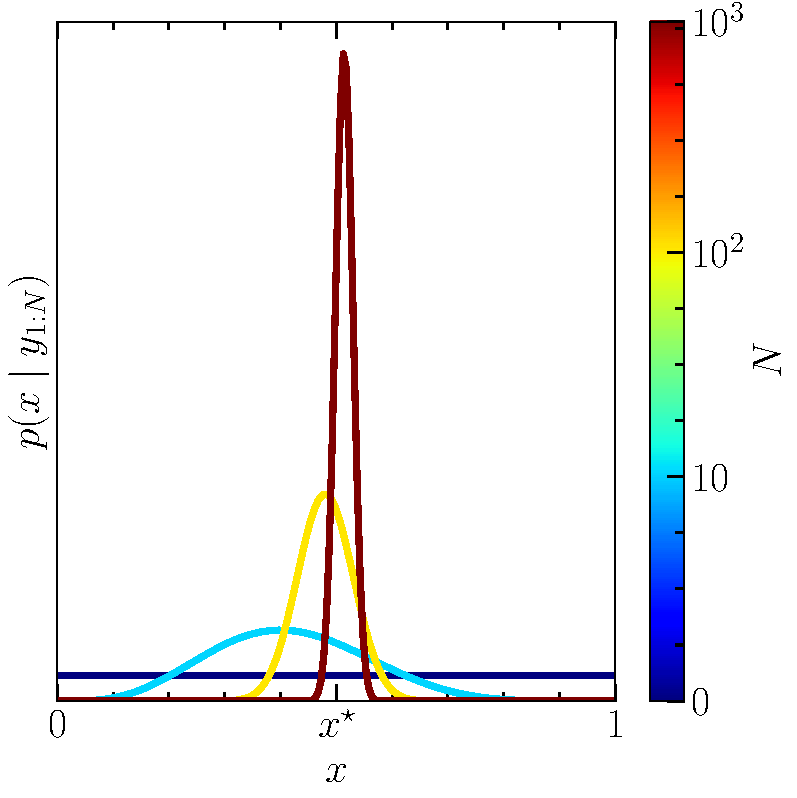
\includegraphics[width=0.4\textwidth]{notebooks/toy_coin_toss.pdf}
        \caption{Exemple d'une inférence bayésienne pour le tirage au sort.}
        \label{fig:bayes update}
\end{figure}

Le lecteur aura compris qu'on va maintenant construire l'apprentissage machine sur des fondations bayésiennes. Ce n'est pas la seule façon de le 
faire. En particulier, il est possible de poser des fondations fréquentistes en supposant, comme fait dans cette section, que toute l'information 
concernant un problème est contenu dans la loi de vraisemblance. Autrement dit, on suppose une ignorance complète \textit{a priori} sur les paramètres d'intérêts. 
En ce sens, et strictement dans le contexte qui nous intéresse, il est possible de passer d'un point de vue à l'autre, puisque les deux théories seront en accord 
sur la réponse à condition qu'on utilise une loi uniforme pour représenter nos connaissances \textit{a priori} sur les paramètres d'intérêts. 
À cause de cette correspondance approximative entre les deux théories, les lois 
\textit{a priori} vont parfois être abandonnées sans justification dans le texte qui suit. 
Le lecteur comprendra qu'on aura simplement changer de point de vue. 

\section{Un exemple d'apprentissage machine: la régression}\label{sec:app classique}

L'apprentissage machine est un concept assez général qui décrit le processus d'extraire l'information contenue 
dans un ensemble de donnée $\mathcal{D} = \{y_i\}_{i=1}^{N}$, soit un ensemble d'observations provenant d'une source ou d'un processus 
physique quelconque. Le terme \textit{information} est utilisé de façon très vague ici. Ce terme est formellement définit dans la théorie 
de l'information de \citet{Shannon1948} comme étant le nombre minimal de \textit{bits} pour décrire une observation $y_i$, ou encore 
l'ensemble de données $\mathcal{D}$. Cette quantité est intimement liée avec l'entropie. Une discussion plus détaillée est 
repoussée au chapitre \ref{chap:intro ml 2}.

Il y a quatre ingrédients essentiels à l'apprentissage machine, soit
\begin{enumerate}
        \item Un ensemble de données $\mathcal{D}$
        \item Un ensemble d'hypothèses $\mathcal{H}_\theta$
        \item Une fonction objective $\mathcal{L}_\theta$
        \item Un algorithme d'optimisation $\mathcal{G}$
\end{enumerate}
Dans cette section, je décrit chacun de ces ingrédients dans le contexte d'une tâche de régression.
La régression est une tâche d'apprentissage machine qui consiste à entraîner un modèle, $f_{\theta}$, sur un ensemble de données augmenté pour la régression, soit 
$\mathcal{D} = \{(x_i, y_i)\}_{i=1}^N$. Chaque exemple dans l'ensemble de donnée est constitué d'un paramètre physique, $x$, et d'une observation, $y$. 
On suppose toujours que les exemples de l'ensemble de données sont générés de façon identiques et indépendantes par la combinaison 
d'une loi \textit{a priori} sur les paramètres physiques et une loi de vraisemblance pour les observations
\begin{equation}
                x \sim p(x),  &\hspace{1cm} y\ \sim p_\theta(y \mid x) \, . 
\end{equation}
Dans le texte, on utilisera le terme \textit{modèle physique} pour faire référence à $p_\theta(y \mid x)$, puisque cette loi de probabilité relie les paramètres physiques, $x$, 
avec les observations, $y$. Elle encodera donc tous les processus physiques en jeu pour un problème d'inférence donné.
On notera de plus que l'ensemble des points de données n'a pas besoin d'être un nombre fini. Dans le cas où $N \rightarrow  \infty$, alors 
$\mathcal{D}$ est explicitement décrit par la loi \textit{a priori}, $p(x)$, et le modèle physique $p_\theta(y \mid x)$. 
Dans ce cas, on dira que la loi générative $(x, y) \sim p(x, y)$ est explicite. 
Dans le cas où $\mathcal{D}$ est un nuage de point, avec $N < \infty$, alors on dira que le processus génératif est implicite. 

Pour se fixer les idées, on considère l'exemple  
\begin{equation}\label{eq:loi generative}
        p(x) = \mathcal{U}(a, b), \hspace{1cm} p_\theta(y \mid x) = \mathcal{N}(y \mid f_\theta(x), \sigma^2)\, .
\end{equation}
On a utilisé le symbole $\mathcal{N}(y \mid \mu, \sigma^2)$ pour décrire une loi normale sur $y$ avec comme moyenne $\mu$ et variance $\sigma^2$. 
On doit supposer que les données sont générées à partir d'une solution quelconque 
\begin{equation}
        f_{\theta^{\star}} = 2x^5 - x\, ,
\end{equation}
avec une amplitude de bruit $\sigma=1$. Ce problème est illustré à la figure \ref{fig:toy problem}.
\begin{figure}[ht!]
        \centering
        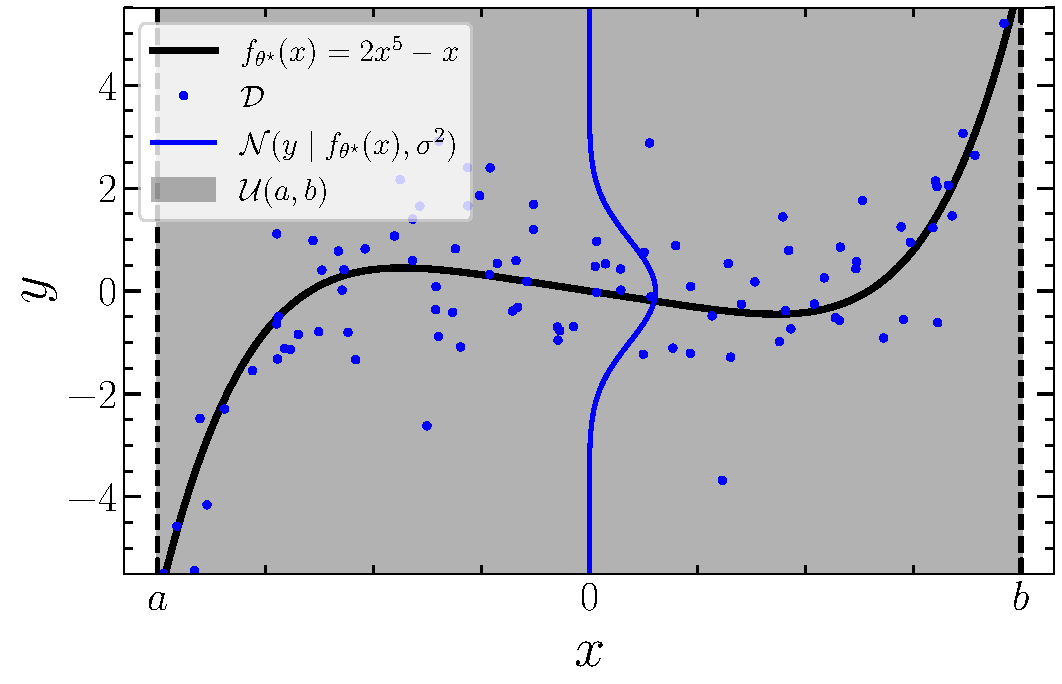
\includegraphics[width=0.5\textwidth]{notebooks/toy_problem}
        \caption{Exemple d'un problème de régression.}
        \label{fig:toy problem}
\end{figure}

Le second ingrédient au problème d'apprentissage machine est la famille des modèles, ou l'ensemble des hypothèses, $\mathcal{H}_\theta$. 
Il serait tentant de choisir le modèle $f_\theta = \theta_1 x^{5} + \theta_2 x$, soit un modèle avec la même forme que la solution 
$f_{\theta^{\star}}$. Toutefois, on ne peut pas assumer que la forme du modèle sera connue \textit{a priori}, 
ou quelle peut facilement être devinée. La sélection du modèle sera abordée en détail dans la section \ref{sec:selection modele}, 
puisque ce sujet mérite une discussion à part entière.
Pour l'instant, on va simplement faire le choix le plus simple en assumant que la forme de 
la loi utilisée pour générer les points de données est inconnue. 
Le choix le plus simple est de construire une famille de modèles linéaires en terme de $x$ et $\theta$
\begin{equation}\label{eq:modele lineaire}
        %\mathcal{H}_\theta = \{f_\theta  \mid f_\theta = \theta_0 + \theta_1 x,\, \theta \in \mathbb{R}^2 \}\, .
        f_\theta = \theta_0 + \theta_1 x%, \hspace{.5cm} \theta \sim p(\theta)
\end{equation} 
Le troisième ingrédient à l'apprentissage machine est de construire une fonction objective pour \textit{entrainer} notre modèle $f_\theta$ sur les points 
de données observés. 
L'objectif de l'entraînement est d'estimer le modèle $f_\theta$, ou de façon équivalente les paramètres $\theta$, qui maximise la loi \textit{a posteriori}, $p(\theta | \mathcal{D})$. En appliquant 
le théorème de Bayes, ceci correspond à
\begin{equation}
        \hat{\theta} = \underset{f_\theta \in \mathcal{H}_\theta}{\mathrm{arg\, max}}\, \frac{p(\mathcal{D} \mid \theta) p(\theta)}{p(\mathcal{D})}
\end{equation} 
Pour faire correspondre cet objectif avec la littérature, on applique le logarithme au côté droit de l'équation, ce qui ne change pas la position des extremas de 
l'objectif, le logarithme étant une fonction monotone. Il est aussi convention de tourner le problème à l'envers, et de chercher plutôt les minimas de la fonction négative. Dans 
ce cas, la fonction objective est
\begin{equation}
        \hat{\theta} = \underset{f_\theta \in \mathcal{H}_\theta}{\mathrm{arg\, min}}\, -\log p(\mathcal{D} \mid \theta) - \log p(\theta) + C(\mathcal{D})\, .
\end{equation} 
où $C(\mathcal{D})$ est une constante qui ne dépend que de l'ensemble de données. L'étape finale est de faire correspondre la vraisemblance $p(\mathcal{D} \mid \theta)$ avec 
le modèle physique, soit la vraisemblance $p_\theta( y \mid x)$. Au travers du texte, les paramètres d'entraînements sont toujours placés en indices, 
par quoi on entend que les paramètres $\theta$ conditionnent la loi de probabilité, $p_\theta(x \mid y) = p(x \mid y, \theta)$. On remarque que
\begin{equation}
        p(\mathcal{D} \mid \theta) = p(x, y \mid \theta) = p(y \mid x, \theta) p(x \mid \theta)\, ,
\end{equation} 
par définition de la loi conditionnelle.  Le dernier terme peut être simplifié en terme de la loi \textit{a priori}, $p(x \mid \theta) = p(x)$ 
puisqu'on suppose que $\theta$ et $x$ sont deux variables aléatoires indépendantes. Un choix de modèle $\theta$ ne devrait pas changer 
la distribution \textit{a priori} sur les paramètres physiques. Si c'est le cas, alors le choix du modèle doit être révisé.
On trouve finalement l'objectif d'entraîenement
\begin{equation}
        \hat{\theta} = \underset{f_\theta \in \mathcal{H}_\theta}{\mathrm{arg\, min}}\, -\log p_\theta(y \mid x) - \log p(\theta) + C(\mathcal{D})\, ,
\end{equation} 
où $-\log p(x)$ est absorbé dans $C(\mathcal{D})$. On est maintenant en mesure de dériver la forme exacte de la fonction objective pour le problème 
posé dans cette section. Avec les suppositions faites plus haut, soit que le modèle physique est une loi normale et que les données sont générées de façon 
$i.i.d$, on a que
\begin{equation}
        \log p_\theta(y \mid x) = \log \prod_{i=1}^{N}p_\theta(y_i \mid x_i) = -\frac{1}{2}\sum_{i=1}^{N}\frac{(y_i - f_\theta(x_i))^2}{\sigma^2} - \frac{N}{2}\log(2\pi \sigma^2)\, ,
\end{equation} 
ce qui correspond à la fonction objective
\begin{equation}\label{eq:MSE intro}
        \hat{\theta} = \underset{f_\theta \in \mathcal{H}_\theta}{\mathrm{arg\, min}}\, \underbrace{ \frac{1}{N}\sum_{i=1}^{N}
        (y - f_\theta(x))^2 }_{\hat{\mathcal{L}}_\theta(\mathcal{D})}  - \frac{2\sigma^2}{N}\log p(\theta)\, .
\end{equation} 
Par convention, on a utilisé le fait que les constantes qui ne dépendent pas de $\theta$ peuvent être ignorées (elles ne changent pas les extremas du problème) 
et on a multiplier la fonction objective par $2\sigma^2 / N$. 
L'expression obtenue fait intervenir la fonction objective approximative $\hat{\mathcal{L}}_{\theta}(\mathcal{D})$, soit un estimé Monte Carlo de l'espérance de l'erreur 
quadratique. En prenant la limite $N \rightarrow \infty$, l'estimé Monte Carlo de l'espérance devient exacte
\begin{equation}
        \lim\limits_{N \rightarrow \infty}\hat{\mathcal{L}}(\mathcal{D}) = \mathcal{L}_{\theta}(\mathcal{D}) = \mathbb{E}_{(x, y) \sim \mathcal{D}} \big[(y - f_\theta(x))^2\big]\, .
\end{equation} 
Dans la littérature, $\hat{\mathcal{L}}_\theta(\mathcal{D})$ est nommée l'erreur quadratique moyenne. Dans le reste de ce mémoire, on va laisser 
tomber le chapeau sur la fonction objective pour simplifier la notation. Le lecteur comprendra qu'on travail généralement avec l'estimé 
Monte Carlo si l'espérance mathématique n'est pas accessible par calcul direct.

Le dernier ingrédient à l'apprentissage machine est le choix d'un algorithme d'optimisation $\mathcal{G}$ pour résoudre l'équation \eqref{eq:MSE intro}, c.-à-d. déterminer 
$\hat{\theta}$. Les algorithmes d'optimisations pour l'apprentissage profond sont généralement basés sur la descente de gradient stochastique, qu'on peut décrire succinctement 
par la relation de récurrence
\begin{equation}\label{eq:gd}
        \hat{\theta}^{(t+1)} = \hat{\theta}^{(t)} - \gamma_t \grad_{\hat{\theta}^{(t)}} \mathcal{L}_{\hat{\theta}^{(t)}}(\mathcal{D})\, ,
\end{equation} 
$\gamma_t$ est le taux d'apprentissage, généralement choisit comme étant aussi grand que possible, 
sans pour autant rendre instable l'algorithme d'optimisation $\mathcal{G}$. Une discussion plus détaillée est reportée au chapitre \ref{chap:intro ml 2} sur ce sujet.

Lorsque on travail à basse dimensions, il est possible d'obtenir de très bons estimés pour $\mathcal{L}_\theta(\mathcal{D})$. 
Par exemple, la figure \ref{fig:monte carlo L} illustre comment 
la variance des contours de l'estimé Monte Carlo $\mathcal{L}_{\theta}(\mathcal{D})$ diminue en fonction de $N$. 
Les rangées montrent un estimé Monte Carlo pour différent tirage de l'ensemble de donnée $\mathcal{D}$ à partir 
de la loi générative décrite à l'équation \eqref{eq:loi generative}, alors que les colonnes montrent  
des ensemble de données de taille croissante. En particulier, la troisième colonne possède des contours très stables, ce qui 
implique que la descente de gradient va retrouver la même solution $\hat{\theta}$ systématiquement, 
contrairement aux estimés où $N$ est relativement petit. Dans ce cas, la solution obtenu par $\mathcal{G}$ 
dépend fortement de l'ensemble de donné observé; la première colonne est l'exemple le plus frappant de ce phénomène.

\begin{figure}[ht!]
        \centering
        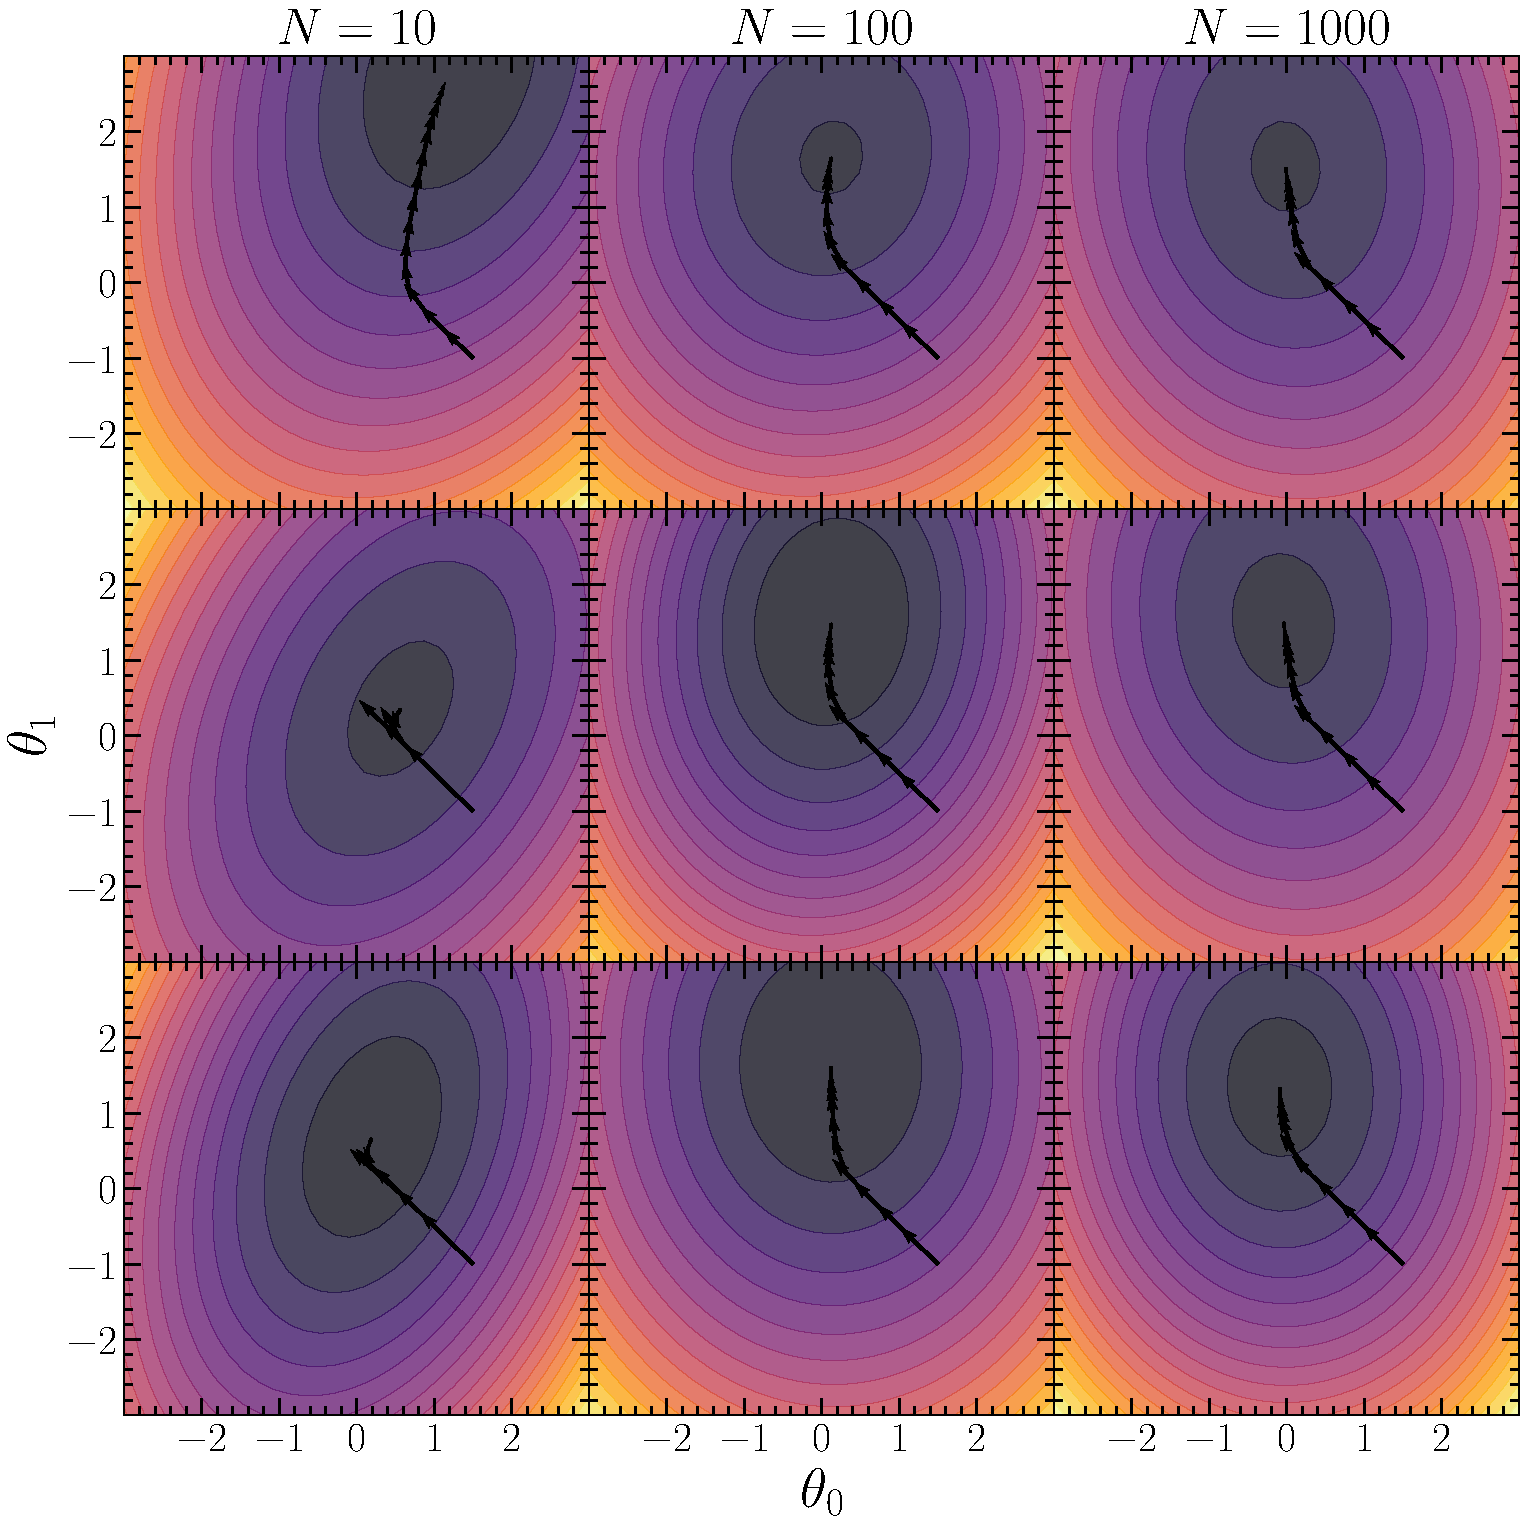
\includegraphics[width=0.7\textwidth]{notebooks/monte_carlo_loss.pdf}
        \caption{Contours de $\mathcal{L}_\theta(\mathcal{D})$ pour différent tirage de $\mathcal{D}$ (rangées) et différentes taille $N = |\mathcal{D}|$ (colonnes) 
                en utilisant le modèle linéaire de l'équation \eqref{eq:modele lineaire} et la loi générative \eqref{eq:loi generative}.
        Une trajectoire produite par la descente de gradient \eqref{eq:gd} est illustré avec les flèches noires.}
        \label{fig:monte carlo L}
\end{figure}

Je termine cette courte introduction avec la définition de deux concepts qui portent parfois à confusion 
dans le jargon de l'apprentissage profond, soit celui d'une \textit{batch} et d'une \textit{époque}.  
Une \textit{batch} $\mathcal{B}$ est un sous ensemble de $\mathcal{D}$, soit $\mathcal{B} \subseteq \mathcal{D}$. Dans le même ordre d'idée du paragraphe précédent, les fonctions objectives 
estimées à partir de différentes \textit{batch}, $\mathcal{L}(\mathcal{B})$, peuvent varier de manière significative entre chaque \textit{batch}. 
Toutefois, sous certains conditions, une descente stochastique avec \textit{batch} est équivalente à une descente de gradient stoachastique avec $\mathcal{L}(\mathcal{D})$, 
soit un estimé à partir de l'ensemble de donnée complet. La descente de gradient stochastique avec \textit{batch} 
est donc particulièrement utile pour l'optimisation de modèles où les données traitées sont de très haute dimensions, 
une situation où l'obtention de la quantité $\mathcal{L}(\mathcal{D})$ requiert souvent une quantité d'opérations machines prohibitive, contrairement à $\mathcal{L}(\mathcal{B})$.
D'un autre côté, une \textit{époque} est un concept assez artificiel qui n'est pas réutilisé dans le reste de ce mémoire. Ce concept correspond à un 
certains nombre d'itérations de la descente de gradient après lequel on aurait épuisé l'ensemble de donné, soit $T = \frac{|\mathcal{D}|}{|\mathcal{B}|}$, 
en assumant que les \textit{batch} sont des sous ensembles distincts de $\mathcal{D}$. 

Ceci complète donc cette introduction à l'apprentissage machine. 
Pour les besoins de ce mémoire, les quelques thèmes abordés ici seront suffisant
pour donner une compréhension à haut niveau des méthodes développées dans les prochains chapitres. Bien sûr, 
cette introduction n'est pas exhaustive. Un lecteur intéressé devrait se référer au références mentionnées au début du 
chapitre.
Les sections qui suivent s'intéresseront à introduire et motiver l'apprentissage profond.


\section{Sélection du modèle}\label{sec:selection modele}

Pour motiver l'apprentissage profond, on s'intéresse maintenant au problème de la sélection du modèle. 
La sélection d'un modèle linéaire à la section précédente n'était motivée que par un critère de simplicité, et en général 
ce critère est insuffisant pour extraire toute l'information qu'un ensemble de donnée contient, ce peut importe les transformations appliquées 
aux espaces $\mathcal{X}$ et $\mathcal{Y}$. Par exemple, un polynôme avec un seul terme (monôme) comme $f_{\theta^{\star}}(x) = Cx^{\alpha}$ peut naturellement être modélisée 
par un modèle linéaire après la transformation approprié de l'espace des paramètres physiques $\mathcal{X} \rightarrow  \log \mathcal{X}$, de sortes 
que le monôme dans le nouvel espace, $f'_{\theta^{\star}} = \alpha \log x + \log C$, est une fonction de forme linéaire en terme de $\alpha$, $\log C$ et $x$.
En général, le prétraitement des données est un aspect important de l'apprentissage machine puisqu'il permet d'éplucher les couches 
de complexités artificielles autour d'un problème d'apprentissage machine donné.

Or, la fonction introduite à la section précédente est déjà un exemple qui ne peut pas être recouvert par un modèle linéaire puisque 
$f_{\theta^{\star}} = 2x^{5} - x$ est un polynôme composé de deux monômes. Minimalement, deux modèles linéaires serait donc nécessaire pour recouvrir $f_{\theta^{\star}}$.
Au mieux, un modèle linéaire est une bonne approximation de $f_{\theta^{\star}}$ pour des régions spéciales du domaine de la fonction comme $|x| \ll 1$ ou $|x| \gg 1$.
On doit donc considérer des modèles plus complexes que le simple modèle linéaire considéré jusqu'à maintenant.

Pour ce faire, il y a trois directions principales. La première méthode, déjà mentionnée dans la section précédente, est de construire une fonction avec la bonne forme \textit{a priori} via l'intuition 
ou possiblement plusieurs décennies de recherche pour les problèmes plus complexe. 
On ne considéra pas plus longtemps cette approche, puisqu'elle est impraticable dans les cas les plus généraux comme les problèmes à haute dimensions où l'intuition humaine échoue complètement.
La seconde approche, et probablement l'approche la plus intuitive considérant la façon dont le sujet a été introduit jusqu'à maintenant, est de considérer une expansion en puissance.
Puisque c'est une approche importante en apprentissage machine, il vaut la peine de dire quelque mots sur celle-ci avant de poursuivre vers la troisième 
et dernière approche possible. 

\subsection{Expansion en puissance pour le cas $x \in \mathbb{R}$}
Lorsque $x \in \mathbb{R}$, l'expansion en puissance prend la forme très simple
\begin{equation}\label{eq:power law}
        f_\theta(x) = \sum_{p = 0}^{P} \theta_p x^{p}\, .
\end{equation} 
%On notera $\mathcal{H}_P$ l'ensemble des polynômes de degré $P$ pour la discussion qui suit.
Le modèle \eqref{eq:power law} est une fonction linéaire en terme des paramètres $\theta$ et non-linéaire en terme des paramètres physiques $x$ ($P > 1$). Dans la limite où $P \rightarrow \infty$, ce modèle 
peut représenter l'ensemble des fonctions analytiques incluant les polynômes, $e^x$, les fonctions trigonométriques, hyperboliques, etc. 

Pour ce cas spécial, on peut explorer comment la complexité du modèle \eqref{eq:power law} influence le problème d'apprentissage. Strictement dans le contexte de l'ajustement 
d'un polynôme $f_\theta: \mathbb{R} \rightarrow \mathbb{R}$ de degré $P < \infty$, la complexité du modèle peut être quantifié par $P$, soit le nombre de termes dans 
l'expansion de puissance. En répétant l'exercice de la section précédente plusieurs fois pour des modèles d'une complexité grandissante,
on peut obtenir des statistiques sur l'erreur de généralisation en fonction de $P$, ce qui est illustré à la figure \ref{fig:bias_variance}.

L'erreur de généralisation est définit comme l'erreur quadratique moyenne d'une fonction calculé sur un ensemble ensemble test, distinct de l'ensemble d'entraînement 
utilisé pour ajuster la fonction.
Cette métrique permet d'estimer le risque encouru lorsqu'on tente d'utiliser une fonction au-delà de son ensemble d'entraînement.
On observe que notre estimé de l'erreur de généralisation atteint un minimum à la complexité $P=5$, ce qui correspond au degrés du polynôme objectif $f_{\theta^{\star}} = 2x^5 - x$. 

%definir erreur de généralisation
\begin{figure}[t]
        \centering
        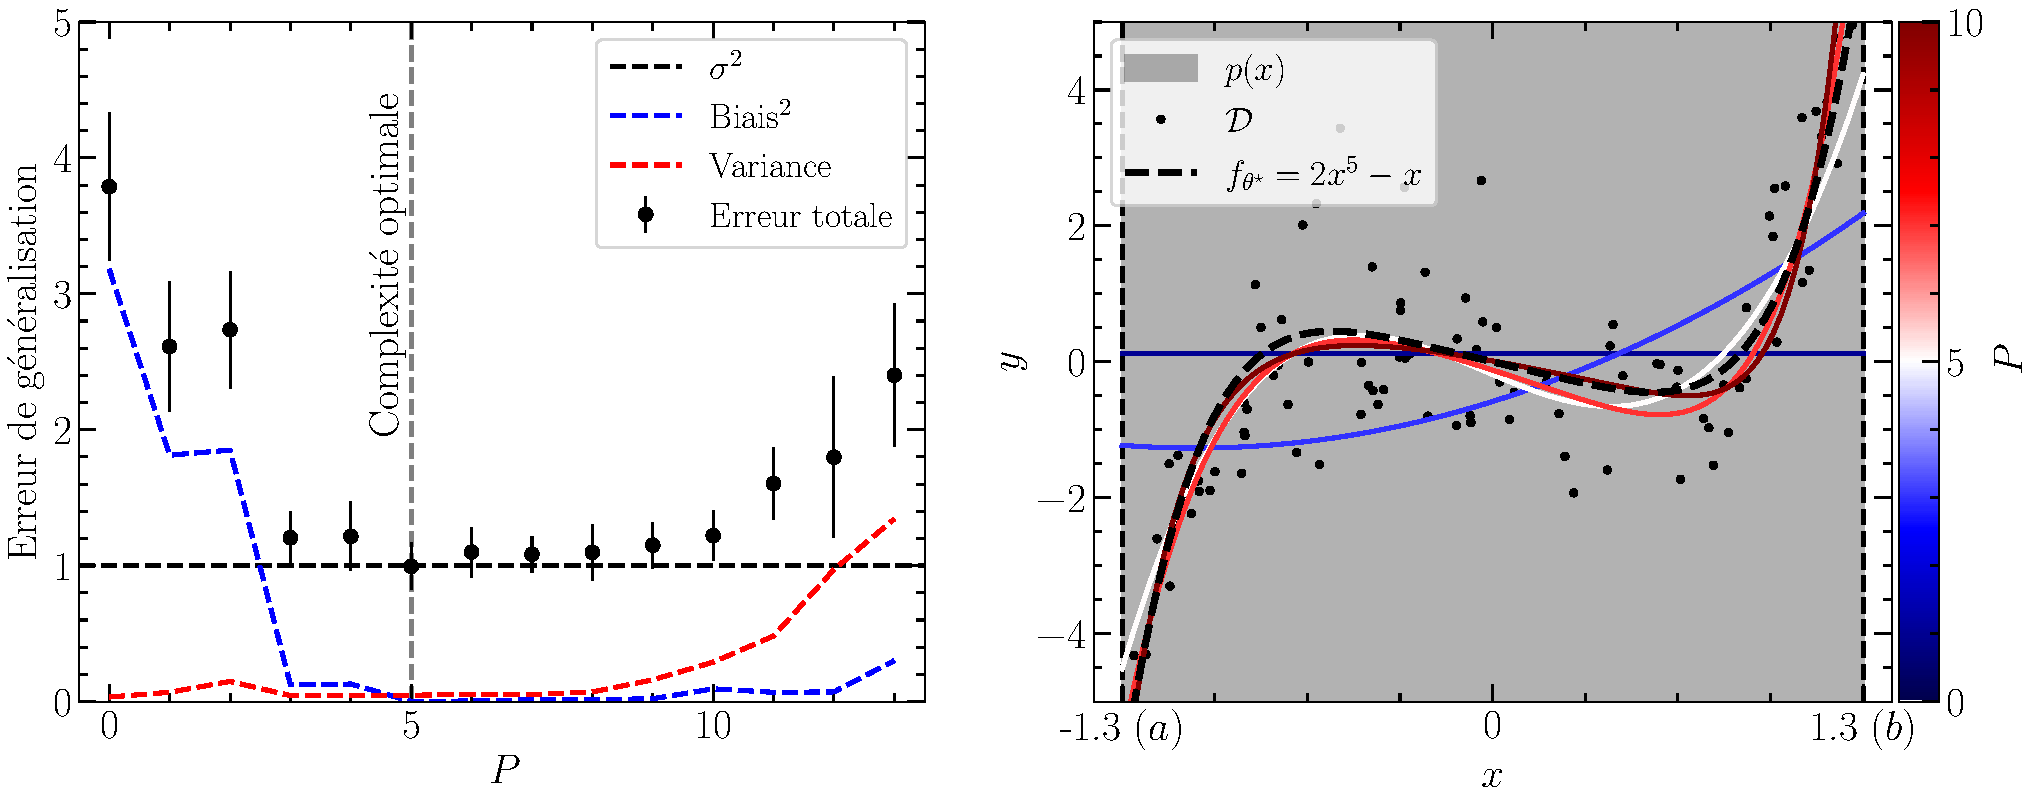
\includegraphics[width=\textwidth]{notebooks/bias_variance.pdf}
        \caption{Compromis classique entre le biais et la variance de d'un algorithme d'apprentissage machine pour l'ajustement d'un polynôme de degré $P$ sur les données générées de la 
        loi $f_{\theta^\star} = 2x^5 - x$.}
        \label{fig:bias_variance}
\end{figure}

Le comportement de cette erreur (en fonction de la complexité du modèle) 
peut être compris intuitivement par une décomposition en terme de l'erreur irréductible du problème 
$\sigma^2$, du biais et de la variance d'un algorithme d'apprentissage machine.
%(voir appendice \ref{app:bias variance} pour une définition formelle de ces termes). 
Lorsque le modèle n'est pas suffisamment complexe pour capturer l'ensemble des points de données, la solution est biaisée par le choix du modèle (courbes bleues de la 
figure \ref{fig:bias_variance}). Le biais est la principale cause du phénomène appelé le \textit{sous-ajustement}, soit lorsqu'un algorithme d'apprentissage n'est pas suffisamment 
flexible pour modéliser une certaine distribution $\mathcal{D}$. Lorsque le modèle est trop complexe, 
le modèle est trop flexible et on observe un phénomène de \textit{sur-ajustement} (courbes rouges de la figure \ref{fig:bias_variance}). Dans ce cas, les modèles entraînés se spécialisent 
à leur ensemble d'entraînement. L'erreur moyenne de généralisation augmente dans cette deuxième situation 
puisque la solution trouvée par l'algorithme d'apprentissage dépend fortement de l'ensemble d'entraînement $\mathcal{D}$.
Dans tous les cas, l'erreur minimale correspond à $\sigma^2$, soit le niveau d'erreur irréductible à un problème donné.

%En général, on s'attend donc à ce qu'un niveau de complexité optimal existe pour un problème donné et qu'il puisse être découvert 
La procédure décrite dans cette sous-section donne une intuition à pourquoi un problème donné requiert un certains niveau de complexité, et 
comment on pourrait potentiellement espérer découvrir cette complexité en terme de l'erreur de généralisation.  
Une discussion formelle de la complexité d'un algorithme requiert une discussion plus avancée. Le lecteur intéressé peut consulter la théorie 
statistique de l'apprentissage machine pour une introduction plus formelle.

\subsection{Expansion en puissance pour le cas $x \in \mathbb{R}^n$}
C'est lorsqu'on cherche à faire une expansion en puissance pour des données multidimensionnelles qu'on réalise que la tâche 
est exponentiellement plus difficile que le cas unidimensionnel. Considérons le cas le plus simple, soit une fonction 
$f_\theta : \mathbb{R}^2 \rightarrow \mathbb{R}$. Dans ce cas, l'expansion en puissance la plus générale est
\begin{equation}\label{eq:multidim expansion}
        f_\theta(x_1, x_2) = \theta^{(0)} 
        + 
        \begin{bmatrix}
                \theta^{(1)}_0 & \theta^{(1)}_1 
        \end{bmatrix}
        \begin{bmatrix}
               x_1 \\
               x_2
        \end{bmatrix}
        +
        \begin{bmatrix}
                x_1 & x_2 
        \end{bmatrix}
        \begin{bmatrix}
                \theta^{(2)}_{11} & \theta^{(2)}_{12} \\
                \theta^{(2)}_{21} & \theta^{(2)}_{22}
        \end{bmatrix}
        \begin{bmatrix}
                x_1 \\ x_2
        \end{bmatrix}
        + \dots
\end{equation} 
% Curse of dimensionality
Le lecteur notera que le terme suivant est une expression qui introduit un tenseur de paramètres $\theta^{(3)}_{ijk}$, soit une tenseur de rang $3$. En général, 
on doit introduire un tenseur de rang $p$ pour le $p^{\text{ième}}$ terme dans l'expansion de puissance, soit $2^p$ nouveaux paramètres qui doivent être ajusté. Dans 
le cas général $f_\theta: \mathbb{R}^n \rightarrow \mathbb{R}^m$, on parle de $n^pm$ nouveaux paramètres pour chaque termes ajoutés dans l'expansion. On comprend donc 
que l'expansion en puissance n'est pas une approche valide pour construire des modèles complexes en haute dimension, puisque le nombre de paramètres introduit 
pour chaque terme dans l'expansion augmente de façon exponentielle. On peut toutefois construire 
un peu d'intuition basé seulement sur le terme d'ordre $2$ dans l'expansion de l'équation \eqref{eq:multidim expansion} pour voir comment on peut construire une approche alternative 
pour augmenter la complexité de nos modèles.




%Toutefois, l'ensemble des  w
%fonctions analytique est un ensemble trop restreint pour résoudre les problème les plus générals. L'exemple le plus simple pour lequel cette approche échoue complètement est 
%la fonction logique XOR, qu'on peut représenter avec la table binaire \ref{tab:xor}.
\begin{table}[H]
        \centering
        \begin{tabular}{ccc}
                $x_1$ & $x_2$ & $f_{\theta^{\star}}(x_1, x_2)$  \\\hline
                0 & 0 & 0 \\ 
                0 & 1 & 1 \\
                1 & 0 & 1 \\
                1 & 1 & 0 \\\hline
        \end{tabular}
        \caption{Fonction logique XOR.}
        \label{tab:xor}
\end{table}

% Fonctione lineaire output w = (0, 0) et b = 1/2 lol.

%En général, la complexité (minimal) requise par un problème d'inférence, particulièrement en haute dimension, f
%Bien qu'un tel critère 
%soit tout à fait justifié par le principe du rasoir d'Occam, on doit tout de même développer une théorie où le critère de simplicité est quantifié, ce pour éviter 
%une situation où la simplicité ajoute des biais non-nécessaire à l'inférence. Autrement dit, on cherche un algorithme d'apprentissage machine qui introduit un niveau minimal 
%de complexité, sans pour autant échouer à modéliser les données correctement (comme c'était le cas à la section précédente).

% Need to do 2 things here, generalize to multi dimensional data, and add complexity.
% Make sure you transmit the point that our point hold up to any transformation of the data (e.g. you can fit an exponential with a linear model).

\section{L'apprentissage machine profond}\label{sec:app profond}

\section{Les réseaux neuronaux convolutifs}\label{sec:cnn}

\paragraph{Overfitting vs Underfitting}

%\paragraph{Taille du dataset vs dimensionalité}
%\paragraph{Intuition pour les problèmes à haute dimensions}

%\subsection{Apprentissage sur des images}
%\paragraph{Introduire un exemple}
Supposons l'exemple de Galaxy Zoo. La tâche est d'extraire de l'information pertinente par rapport à l'Univers,e 
la formation des galaxies et tout autre phénomène d'intérêts pour les astrophysicens. Or, on a seulement accès à des images 
provenant de téléscopes sur Terre des ces galaxies. Clairement, ces dizaines de milliers d'images contiennent une richesse 
énorme d'information, mais comment extraire l'information pertinente à une tâche en particulier?

L'idée est de comprimer toute cette information à quelques features qui décrivent ces galaxies de façon pertinente. Les clases choisit sont xyz. 
Et l'approche choisit a été de recruté des milliers de citoyens volontaires pour regarder au traves des centaines de milliers d'images, quelles sont celle qui contiennent 
les feature que les scientifiques ont décidé été intéressantes. 

Est-ce que c'est la bonne approche? Clairement, cela demande beaucoup d'effort. 

Est-ce que sont les meilleurs features? Cela va dépendre de la science. Pour d'autre science, cette compression sera loin d'être optimale.

Une autre approche de compression est du supposer un modèle constituer de quelques paramètres, qu'on peut étudier plus facilement. Par exemple, supposons une 
Sersic. On peut fitter ce modèle à toutes les galaxies dans notre dataset, et puis étudier l'ensemble des paramètres obtenus comme 
compression de l'information pour faire la science qui nous intéresse, par exemple étudier la taille apparente des galaxies en fonction du redshift pour 
étudier la cosmologie.

Cette seconde approche est un peu plus intéressante, car elle est plus efficace. Toutefois, on retrouve encore une fois le problème mentionné plus 
haut où la taille de notre ensemble d'hypothèse, ici $\mathcal{H}_\theta$ est l'ensemble des profils 2D qui peuvent être construit par une fonction Sérsic, 
limite sévèrement l'expressivité la qualité de nos fit, et le type de conslusions qu'on peut en tirer. En particulier, est-ce que notre compression va 
biaiser notre inférence etc.

Alors que peut-on faire? On aimerait combiner les deux approches précédentes. C-à-d. somehow avoir une fonction qui peut regarder des images et 
inférer l'information qui nous intéresse pour notre science. Regardons de plus près quelle devrait être cette fonction. 

Blablabla, on réalise qu'on peut induire de l'information dans cette fonction. En particulier, notre réponse ne devrait pas changer si on 
applique une translation à l'image. Cette symétrie induit une convolution. Bien qu'on pourrait dire quelque chose de smiliare pour les rotations, 
il est beaucoup plus difficile de construire une fonction invariante sous rotation, donc on s'arrête ici. 

Maintenant on s'intéresse à agrandir notre ensemble d'hypothèse pour inclure le plus d'hypothèse possibles, de sortes que la loi la plus efficace possible, $f^{\star}$, 
qu'on suppose existe, puisse être découverte par notre algorithme d'optimisation.
\paragraph{Les réseaux convolutionnels}
Comment introduire les réseaux de neuronnes convolutionnels, maintenant qu'on sait comment construire un réseau de neuronnes simple? 
En fait, on peut remarquer que nos réseaux de neuronnes simples ne scale pas à haute dimensions. En effet, les hypothèses générales qu'on a fait 
pour obtenir un approximateur universel sont qu'on doit apprendre chaque connections entre l'input et l'output d'une layer du réseau. Le nombre de 
dimensions pour des images approche rapidement les dizaines de milliers, voir des millions. Clairement, le nombre de paramètre va gradir très rapidement et 
la complexité du modèle sera compliqué. 

L'idée est d'exploiter les symétries du problème, de la même façon qu'on sait le faire en mécanique classqieu avec le théorème de Noether. 
Dans ce cas, exploiter une symétrie revient à introduire un biais inductif dans le problème qui vient restreindre énormément l'ensemble $\mathcal{H}_\theta$. 
Cela peut sembler contre-intuitif, puisqu'on vient de dire qu'on cherchais à agrandir $\mathcal{H}_\theta$, mais voyons comment cela peut nous être utile. 

Supposons la tâche de classifier les images de Galaxy-Zoo en galaxies spirales ou non spirales. La fonction la plus bête qu'on peut construire 
est un modèle linérair qui fait une somme moyenné par des poids appris de chaque pixels vers les deux catégories qui nous-intéressent. On 
utilise un scheme one-hot encoding pour les deux catégories, donc $y = [0, 1]$ pour les galaxies spirales, et $y = [1, 0]$ pour les galaxies non-spirales 
let's say. Alors, on utilise encore notre MSE précédente, et on utilise le framework de régression logistique, voulant dire qu'on cherche a à prédire 
la probabilité qu'une galaxie soit une des deux catégorie, avec la somme des probabilité normalisé.

Ok, dans ce scheme, on peut comprendre que déplacer, faire une trranslation, de l'image ne devrait pas changer le résultat de la prédiction. 
Ainsi, on a une fonction qui doit être invariant sous translation de l'image
\begin{equation}
        \begin{split}
                x &\rightarrow Tx \\
                f_\theta(x) &\rightarrow f'_\theta(Tx) = f_\theta(x)
        \end{split}
\end{equation} 
Donc le résultat ne devrait pas changer. Ici, on essaie de construire une fonction qui respecte cette condition. Donc on veut construire $\mathcal{H}_\theta$ 
qui ont cette symétrie. Quels type de fonction ont cette symétrie?

Build an example where you show that you want the same weight everywhere. Also that pooling operations are allowed. Generalize to 2D. Make connection with 
convolutions.


\paragraph{L'architecture sablier}
\paragraph{L'architecture en U}
\paragraph{Contrôler les biais inductifs}
\paragraph{Contrôler l'expressivité}
%Example, Galaxy Zoo

% Refer to Bengio's intro to ML, Bishops and Murphy.

%Plan
%-> A probabilistic intro to ML
        %-> Why do model learn the mean?
%-> Introduce some standard architectures for images
%-> Introduce the concepts of a dataset, test set, loss or objective, empirical risk
%-> Why even go to super large models?
%-> Introduce stochastic gradient descent and recent approach to it
%-> Preprocessing, whitening the data?
%-> Activation functions and their role?


